\section{T-I: Push-T Results}

\subsection{Configuration}

Table~\ref{tab:pusht-config} records the resolved configuration used by the reportable run. It is
saved with the checkpoints rather than reconstructed from command history.

\begin{table}[t]
    \centering
    \caption{Reportable Push-T training configuration.}
    \label{tab:pusht-config}
    \footnotesize
    \begin{tabular}{@{}p{0.62\linewidth}R{0.29\linewidth}@{}}
        \toprule
        Setting & Value \\
        \midrule
        Training seed / RGB demonstrations & 1 / 100 \\
        Transitions / windows & 9,865 / 9,765 \\
        Observation / action / prediction horizon & 2 / 1 / 16 \\
        Diffusion steps & 100 \\
        U-Net widths & $[64,128,256]$ \\
        Spatial visual feature dimension & 256 \\
        Batch size / learning rate & 128 / $10^{-4}$ \\
        Warmup / total updates & 500 / 50,000 \\
        Maximum episode steps & 150 \\
        Backend / controller & GPU PhysX / delta pose \\
        Dataset device / policy device & CPU / CUDA \\
        \bottomrule
    \end{tabular}
\end{table}

\subsection{Training dynamics and checkpoint selection}

Figure~\ref{fig:pusht-results} summarizes the optimization and evaluation evidence. The
1,000-step moving-average diffusion loss decreases from 0.0533 at iteration 11k to 0.0183 at 50k.
The raw logged loss at 50k is 0.0274. This establishes optimization progress, but it does not
identify the best controller: diagnostic \successonce peaks at 30\% at 15k, drops to 10\% at
25k, and returns to 30\% at 40k even as loss continues to decrease.

The selected checkpoint is therefore the EMA policy at iteration 15k. The 40k score ties rather
than exceeds the first maximum, and the implementation intentionally requires strict improvement.
This avoids silently changing a selected checkpoint on an equal, noisy 20-episode estimate.

\begin{figure*}[t]
    \centering
    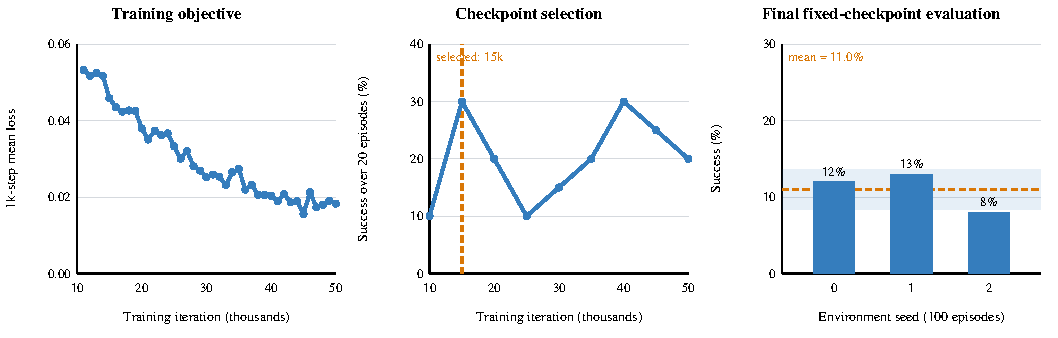
\includegraphics[width=0.99\textwidth]{fig/pusht_ti_results.pdf}
    \caption{\textbf{Left:} diffusion loss logged every 100 updates and summarized by a trailing
    1,000-step mean. The original 0--10k Colab event file was not preserved, so the trace begins at
    10.1k. \textbf{Center:} 20-episode \successonce diagnostic used only for checkpoint selection;
    the dashed marker is the selected 15k checkpoint. \textbf{Right:} reportable evaluation of
    that fixed checkpoint over 100 fresh rollouts per seed. The line and band denote the
    three-seed mean and one sample standard deviation.}
    \label{fig:pusht-results}
\end{figure*}

\subsection{Fixed-checkpoint baseline}

Table~\ref{tab:pusht-eval} reports the required 300-rollout evaluation. The fixed 15k checkpoint
achieves \tiseedzero, \tiseedone, and \tiseedtwo{} \successonce for seeds 0, 1, and 2. The
three-seed baseline is \textbf{\timean\% $\pm$ \tistd{} percentage points}, with \tipooled{}
pooled successes. The corresponding mean \successend is \timeanend\%.

\begin{table}[t]
    \centering
    \caption{Fixed 15k checkpoint; 100 Push-T rollouts per environment seed.}
    \label{tab:pusht-eval}
    \footnotesize
    \setlength{\tabcolsep}{4pt}
    \begin{tabular}{@{}lrrrr@{}}
        \toprule
        Seed & Once & End & Max ov. & Final ov. \\
        \midrule
        0 & \tiseedzero & \tiseedzeroend & \tiseedzeromax & \tiseedzerofinal \\
        1 & \tiseedone & \tiseedoneend & \tiseedonemax & \tiseedonefinal \\
        2 & \tiseedtwo & \tiseedtwoend & \tiseedtwomax & \tiseedtwofinal \\
        \midrule
        Mean & \timean\% & \timeanend\% & -- & -- \\
        Sample std. & \tistd{} pp & \tistdend{} pp & -- & -- \\
        \bottomrule
    \end{tabular}
\end{table}

The final estimate is lower than the 30\% selection diagnostic. This is not a contradiction: the
diagnostic contains only 20 episodes and was repeatedly queried during training, while each final
seed contains 100 fresh episodes. The larger evaluation is the baseline; the diagnostic is only a
checkpoint-selection instrument. A nonzero gap between \successonce and \successend also captures
policies that reach 0.90 overlap transiently and subsequently displace the block.

\subsection{Training time and resource use}

The first 10,000 updates were trained in Colab, but the Colab start timestamp was not preserved;
we therefore do not invent an end-to-end wall time. The measured Runpod continuation from 10k to
15k takes 16 min 27 s including its diagnostic evaluation. After a process termination, the
checkpoint-complete 15k--50k continuation takes 2 h 2 min 35 s, also including seven scheduled
20-episode evaluations. The total observed 10k--50k continuation is 2 h 19 min 2 s.

For the uninterrupted 15k--50k segment, \texttt{nvidia-smi} was sampled every 5 s for 1,475
measurements. On one 46,068 MiB NVIDIA A40, peak sampled allocation is 7,603 MiB (7.42 GiB), peak
sampled utilization is 54\%, and peak sampled power is 187.93 W. ``Sampled'' is essential: these
are observations at discrete times, not guaranteed instantaneous maxima.
